\documentclass[12pt]{article}
\usepackage{amsmath,amssymb}
\usepackage{mathtools}
\usepackage{hyperref}

\usepackage{tikz}
\usepackage{cancel}

\usetikzlibrary{decorations.pathreplacing}

\title{Approximating the Period of a Pendulum\\[0.2em]
\large AP Calculus BC: Taylor Series Project}
\author{Andrew Chou \and Kevin Ma \and James Tsaggaris}

\linespread{1.25}
\setlength{\skip\footins}{3\baselineskip}   % Adjust space between
% text and footnotes

\begin{document}

\maketitle

\begin{center}
  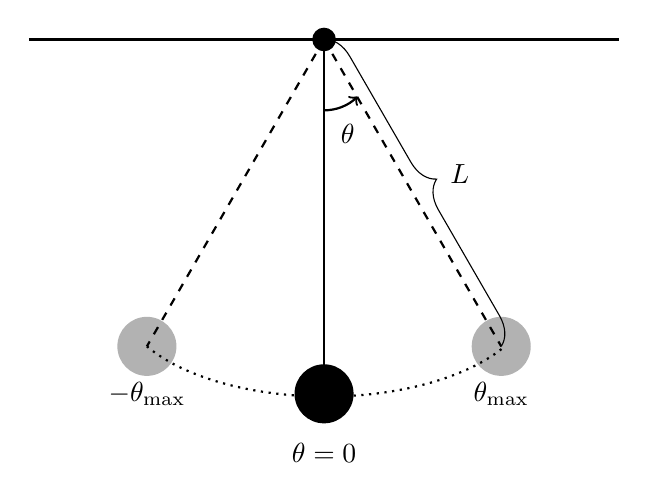
\begin{tikzpicture}[scale=1.5]
    % Draw ceiling
    \draw[thick] (-2.5,3) -- (2.5,3);

    % Draw pivot point
    \fill[black] (0,3) circle (0.1);

    % Calculate pendulum length (3 units)
    \def\pendulumLength{3}

    % Draw pendulum at equilibrium position (vertical)
    \draw[thick] (0,3) -- (0,{3-\pendulumLength});
    \fill[black] (0,{3-\pendulumLength}) circle (0.25);

    % Draw left swing position (30 degrees)
    \draw[thick,dashed] (0,3) --
    ({-\pendulumLength*sin(30)},{3-\pendulumLength*cos(30)});
    \fill[black,opacity=0.3]
    ({-\pendulumLength*sin(30)},{3-\pendulumLength*cos(30)}) circle (0.25);

    % Draw right swing position (30 degrees)
    \draw[thick,dashed] (0,3) --
    ({\pendulumLength*sin(30)},{3-\pendulumLength*cos(30)});
    \fill[black,opacity=0.3]
    ({\pendulumLength*sin(30)},{3-\pendulumLength*cos(30)}) circle (0.25);

    % Draw connecting arc for the path
    \draw[thick,dotted]
    ({-\pendulumLength*sin(30)},{3-\pendulumLength*cos(30)}) arc
    (-150:-30:1.75 and 0.85);

    % Draw angle theta (to right swing position)
    \draw[->,thick] (0,2.4) arc (-90:-45:0.4);
    \node at (0.2,2.2) {$\theta$};

    % Label theta max at the right swing position
    \node at (1.5,0) {$\theta_{\mathrm{max}}$};

    % Label negative theta max at the left swing position
    \node at (-1.5,0) {$-\theta_{\mathrm{max}}$};

    % Label equilibrium position
    \node at (0,-0.5) {$\theta = 0$};

    % Oblique overbrace representing L for the right pendulum
    \draw[decorate,decoration={brace,amplitude=10pt}] (0,3) --
    ({\pendulumLength*sin(30)},{3-\pendulumLength*cos(30)})
    node[midway,above,xshift=17pt] {$L$};
  \end{tikzpicture}
\end{center}

\section{Inputs}
\begin{itemize}
  \item $L$: Length of pendulum (meters)
  \item $\theta_{\mathrm{max}}$: Maximum angular displacement (radians)
\end{itemize}

\section{Period of a Pendulum}
\[
  T = 2\pi \sqrt{\frac{L}{g}} \int_{0}^{\frac{\pi}{2}} \frac{1}{\sqrt{1 - k^2
  \sin^2 \theta}} \, d\theta
\]
where $k = \sin\left(\frac{\theta_{\mathrm{max}}}{2}\right)$ (a constant).

\section{Series Expansion}
Let $u = k^2 \sin^2 \theta$, and the integrand becomes:
\[
  f(u) = \frac{1}{\sqrt{1 - u}} = (1 - u)^{-\frac{1}{2}}
\]
which is in the form of a binomial series $(1+x)^k =
\sum_{n=0}^{\infty} \binom{k}{n} x^n$.

Since we have not yet covered binomial series in class, we will instead
use the Maclaurin series expansion for $(1 - u)^{-1/2}$ around $u =
0$. First, we find the general form of the $n$th derivative:
\begin{align*}
  f^{(0)}(u) &= (1-u)^{-\frac{1}{2}} &&\rightarrow f^{(0)}(0) =
  \frac{1}{\cancel{2^0}} \\
  f^{(1)}(u) &= -\frac{1}{2} (1-u)^{-\frac{3}{2}} &&\rightarrow
  f^{(1)}(0) = -\frac{1}{2^1} \\
  f^{(2)}(u) &= \frac{1\cdot3}{2^2} (1-u)^{-\frac{5}{2}}
  &&\rightarrow f^{(2)}(0) = \frac{1\cdot3}{2^2} \\
  f^{(3)}(u) &= -\frac{1\cdot3\cdot5}{2^3} (1-u)^{-\frac{7}{2}}
  &&\rightarrow f^{(3)}(0) =
  {\color{violet}\underbrace{-}_{\mathclap{\text{alternating}}}}
  \frac{\color{blue}\overbrace{1\cdot3\cdot5}^{\mathclap{\text{odd-only
  factorial}}}}{\color{red}2^3} \\
  f^{(n)}(u) &= \frac{{\color{blue}(2n-1)!!}}{{\color{red}2^n}}
  {\color{violet}(-1)^n}
\end{align*}

Plugging in to the Maclaurin series formula $f(x) =
\sum_{n=0}^{\infty} \frac{f^{(n)}(0)}{n!} x^n$, we get:
\[
  \frac{1}{\sqrt{1 - u}} = \sum_{n=0}^{\infty} \frac{(-1)^n
  (2n-1)!!}{2^n n!} u^n
\]
Since $2^n n!$ is equivalent to multiplying by 2 for every term in
the factorial, we can rewrite the series as the following, after
substituting $u = k^2 \sin^2 \theta = (k\sin\theta)^2$:
\[
  \sum_{n=0}^{\infty} \frac{(-1)^n (2n-1)!!}{(2n)!!}
  {\left(k\sin\theta\right)}^{2n}
\]
Keep in mind that for $n = 0$, $(2(0) - 1)!! = (-1)!! = 1$ by
convention. \footnote{\url{https://mathworld.wolfram.com/DoubleFactorial.html}}

\section{Simplifying the Integral}

Substitute the above Maclaurin series into the integral:
\[
  \int_{0}^{\frac{\pi}{2}} \frac{1}{\sqrt{1 - k^2
  \sin^2 \theta}} \, d\theta = \int_{0}^{\frac{\pi}{2}}
  \sum_{n=0}^{\infty} \left[\frac{(-1)^n (2n-1)!!}{(2n)!!}
  {\left(k\sin\theta\right)}^{2n}\right] \, d\theta
\]
Take constant (non-$\theta$) terms out of the integral, since they
are independent of $\theta$:
\[
  = \sum_{n=0}^{\infty} \left[\frac{(-1)^n (2n-1)!!}{(2n)!!} k^{2n}
  \int_{0}^{\frac{\pi}{2}} \sin^{2n} \theta \, d\theta\right]
\]

We evaluate the first three terms of the series to get a sense of the pattern:
\[
  1 - \frac{1}{2}k^2\int_{0}^{\frac{\pi}{2}} \sin^2 \theta \, d\theta
  + \frac{3}{8}k^4\int_{0}^{\frac{\pi}{2}} \sin^4 \theta \, d\theta + \cdots
\]

Find the values of the definite integrals using half-angle identities:
\[
  \int_{0}^{\frac{\pi}{2}} \left(\frac{1}{2} -
  \frac{1}{2}\cos(2\theta)\right) \, d\theta = \left[\frac{\theta}{2}
  - \frac{1}{4}\sin(2\theta)\right]_{0}^{\frac{\pi}{2}} = \frac{\pi}{4}
\]
\[
  \int_{0}^{\frac{\pi}{2}} \sin^4 \theta \, d\theta =
  \left[\frac{\theta}{4} - \frac{1}{4}\sin(2\theta) +
    \frac{\theta}{8} +
  \frac{1}{32}\sin(4\theta)\right]_{0}^{\frac{\pi}{2}} =
  \frac{\pi}{8} + \frac{\pi}{16} = \frac{3\pi}{16}
\]

The resulting terms are:
\[
  1 - \frac{1}{2}k^2\left(\frac{\pi}{4}\right) +
  \frac{3}{8}k^4\left(\frac{3\pi}{16}\right) + \cdots
\]

The process is tedious, but we see that each integral is in the form
of Wallis integrals, defined by the sequence $W_n =
\int_{0}^{\frac{\pi}{2}} \sin^n \theta \, d\theta$. Evaluating each
definite integral gives some multiple of $\frac{\pi}{2}$, and the
antiderivative of all the recursive cosines from the half-angle
identities all vanish, since $\sin(2n \cdot \frac{\pi}{2}) =
\sin(n\pi) = 0$. Through integration by parts and recursive
substitution of $I$, the value of even Wallis integrals are known to be:
\[
  W_{2n} = \frac{(2n-1)!!}{(2n)!!} \cdot \frac{\pi}{2}
\]

After substituting in the value of the Wallis integrals, we can now express the general (approximate) formula for the period of a pendulum using the integrated Maclaurin series:
\begin{align*}
  T &= 2\pi \sqrt{\frac{L}{g}} \sum_{n=0}^{\infty} \left[\frac{(-1)^n (2n-1)!!}{(2n)!!} k^{2n} \cdot W_{2n}\right] \\
  &= 2\pi \sqrt{\frac{L}{g}} \sum_{n=0}^{\infty} \left[\frac{(-1)^n (2n-1)!!}{(2n)!!} k^{2n} \cdot \frac{(2n-1)!!}{(2n)!!} \cdot \frac{\pi}{2}\right] \\
  &= 2\pi \cdot \frac{\pi}{2} \sqrt{\frac{L}{g}} \sum_{n=0}^{\infty} \left[(-1)^n k^{2n} \left(\frac{(2n-1)!!}{(2n)!!}\right)^2 \right] \\
  &= \pi^2 \sqrt{\frac{L}{g}} \sum_{n=0}^{\infty} \left[(-1)^n \left(\frac{(2n-1)!!}{(2n)!!}\right)^2 k^{2n} \right]
\end{align*}

\end{document}
